\documentclass[12pt]{scrartcl}
\usepackage[sexy]{james}
\usepackage[noend]{algpseudocode}
\setlength {\marginparwidth}{2cm}
\usepackage{answers}
\usepackage{array}
\usepackage{tikz}
\newenvironment{allintypewriter}{\ttfamily}{\par}
\usepackage{listings}
\usepackage{xcolor}
\usetikzlibrary{arrows.meta}
\usepackage{color}
\usepackage{mathtools}
\newcommand{\U}{\mathcal{U}}
\newcommand{\E}{\mathbb{E}}
\usetikzlibrary{arrows}
\Newassociation{hint}{hintitem}{all-hints}
\renewcommand{\solutionextension}{out}
\renewenvironment{hintitem}[1]{\item[\bfseries #1.]}{}
\renewcommand{\O}{\mathcal{O}}
\declaretheorem[style=thmbluebox,name={Chinese Remainder Theorem}]{CRT}
\renewcommand{\theCRT}{\Alph{CRT}}
\setlength\parindent{0pt}
\usepackage{sansmath}
\usepackage{pgfplots}

\usetikzlibrary{automata}
\usetikzlibrary{positioning}  %                 ...positioning nodes
\usetikzlibrary{arrows}       %                 ...customizing arrows
\newcommand{\eqdef}{=\vcentcolon}
\newcommand{\tr}{{\rm tr\ }}
\newcommand{\im}{{\rm Im\ }}
\newcommand{\spann}{{\rm span\ }}
\newcommand{\Col}{{\rm Col\ }}
\newcommand{\Row}{{\rm Row\ }}
\newcommand{\dint}{\displaystyle\int}
\newcommand{\dt}{\ {\rm d }t}
\newcommand{\PP}{\mathbb{P}}
\newcommand{\horizontal}{\par\noindent\rule{\textwidth}{0.4pt}}
\usepackage[top=3cm,left=3cm,right=3cm,bottom=3cm]{geometry}
\newcommand{\mref}[3][red]{\hypersetup{linkcolor=#1}\cref{#2}{#3}\hypersetup{linkcolor=blue}}%<<<changed

\tikzset{node distance=4.5cm, % Minimum distance between two nodes. Change if necessary.
         every state/.style={ % Sets the properties for each state
           semithick,
           fill=cyan!40},
         initial text={},     % No label on start arrow
         double distance=4pt, % Adjust appearance of accept states
         every edge/.style={  % Sets the properties for each transition
         draw,
           ->,>=stealth',     % Makes edges directed with bold arrowheads
           auto,
           semithick}}


% Start of document.
\newcommand{\sep}{\hspace*{.5em}}

\pgfplotsset{compat=1.18}
\begin{document}
\title{AMSC460: Computational Methods}
\author{James Zhang\thanks{Email: \mailto{jzhang72@terpmail.umd.edu}}}
\date{\today}

\definecolor{dkgreen}{rgb}{0,0.6,0}
\definecolor{gray}{rgb}{0.5,0.5,0.5}
\definecolor{mauve}{rgb}{0.58,0,0.82}

\lstset{frame=tb,
  language=Java,
  aboveskip=3mm,
  belowskip=3mm,
  showstringspaces=false,
  columns=flexible,
  basicstyle={\small\ttfamily},
  numbers=left,
  numberstyle=\tiny\color{gray},
  keywordstyle=\color{blue},
  commentstyle=\color{dkgreen},
  stringstyle=\color{mauve},
  breaklines=true,
  breakatwhitespace=true,
  tabsize=3
}


\maketitle
These are my notes for UMD's CMSC460: Computational Methods. These notes are taken live in class 
(``live-\TeX``-ed). This course is taught by Professor Haizhao Yang. The textbook for the course is 
\textit{A First Course in Numerical Methods} by OU Ascher and Chen Greif.
\tableofcontents

\newpage

\section{Scientific Computing}

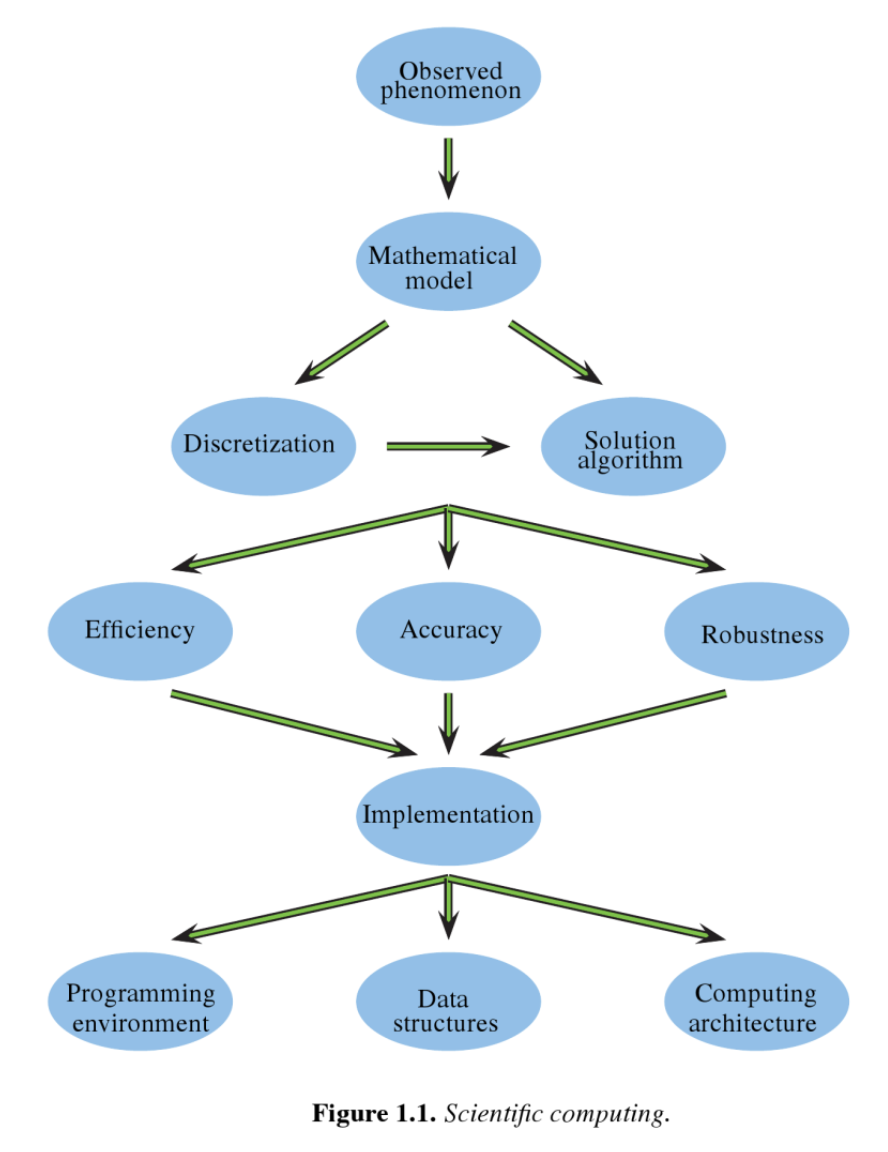
\includegraphics[width=10cm]{scientific_compute.png}

\begin{definition}[Relative and Absolute Errors]
  Let the target value be $u \in \RR$ and let the numerical solution be $v \in \RR$, then the 
  \vocab{absolute error} is $|u-v|$ and the \vocab{relative error} is $\frac{|u-v|}{|u|}$.
\end{definition}

\begin{note}
If $|u|$ is large, then relative error is used and if $|u|$ is very small, then relative error 
is not a good measurement.
\end{note}

\begin{example}[The Stirling Approximation]
  The formula $u = S_n = \sqrt{2\pi n} \cdot(\frac{n}{e})^n$ is used to approximate $n!$.
  \begin{lstlisting}[language=Matlab]
    e = exp(1);
    n = 1 : 10;
    # Note that the following are vectors of len 10.
    S_n = sqrt(2*pi*n).*((n/e).^n);
    # Compute absolute and relative err.
    fact_n = factorial(n);
    abs_err = abs(fact_n - S_n);
    rel_err = abs_err./abs(fact_n);
    format short g
    [n; fact_g; abs_err; real_err;]'
  \end{lstlisting}
\end{example}

\subsection{Numerical Algorithms and Errors}

\begin{definition}[Error Types]

  \hfill

  \begin{enumerate}
    \item Error in the problem to be solved. These may be errors in the mathematical model or errors in the input data.
    \item Approximation errors, which can consist of discretization errors (errors in interpolation, differentiation, integration) or 
    convergence errors, which can also arrive in iterative methods
    \item Roundoff errors
  \end{enumerate}
\end{definition}

\begin{definition}[Taylor Series]
  Assume that $f(x)$ has $k+1$ derivatives in an interval containing the point $x_0$ and 
  $x_0 + k$. Then 
  \[f(x_0 + k) = f(x_0) + hf'(x_0)+ \frac{h^2}{2} + \cdots + \frac{h^k}{k!}f^{(k)}(x_0) + \frac{h^{k+1}}{(k+1)!}f^{(k+1)}(\xi)\]
  where $\xi$ is some point between $x_0$ and $x_0 + h$, and the term $\frac{h^{k+1}}{(k+1)!}f^{(k+1)}(\xi)$ is the remainder term.
\end{definition}

\begin{note}
  To find $f'(x_0)$ observe that 
  \[f'(x_0) = \frac{f(x_0 + k) - f(x_0)}{h}\] 
  and then if we take the limit of this 
  \[f'(x_0) = \lim_{h\to 0} \frac{f(x_0 + k) - f(x_0)}{h}\]
  we recover the $h$-definition of a derivative, and the discretization error is 
  $\frac{h}{2}f''(\xi)$ because our model is 
  \[hf'(x_0) = f(x_0 + k) - f(x_0) - \frac{h^2}{2}f''(x_0) + \cdots\]
  \[\implies f'(x_0) = \frac{f(x_0 + k) - f(x_0)}{h} - \left(\frac{h}{2}f''(x_0) + \cdots\right)\]
  \[\implies \left| f'(x_0) - \frac{f(x_0 + k) - f(x_0)}{h} \right| = \left| \frac{h}{2}f''(x_0) + \cdots \right|\]
\end{note}

\begin{definition}[Big-$\mathcal{O}$ and $\Theta$ Notation]
  We define these for error characterization in terms of some parameters.
  \[\begin{cases}
    h \text{ represents a small parameter }\\
    n \text{ represents a large parameter }
  \end{cases}\]
\end{definition}

\begin{note}
  An error $e$ depending on $h$ we denote $e = \mathcal{O}(h^q)$ and if there are two positive constants 
  $q$ and $C$ such that 
  \[|e| \leq Ch^q\]
  Similarly, we write $e = \Theta(h^q)$ if $\ \exists \ C_1, C_2$ and $q > 0$
  such that 
  \[C_1h^q \leq |e| \leq C_2h^q\]
  $n$ represents the problem size and then we use big $\O$ and $\Theta$ to denote the time or memory complexity of an algorithm.
\end{note}

\begin{example}
  If we say $T = \Theta(n\log n)$ then we find $C_1, C_2, x_0$ such that 
  \[C_1n\log n \leq T \leq C_2n \log n \ \forall \ x \geq x_0\]
\end{example}

\begin{note}
    
  Note that errors go down and then back up as $h$ changes. A small number divided by another small number is a dangerous,
  think about exploding and vanishing gradients when training neural networks.

  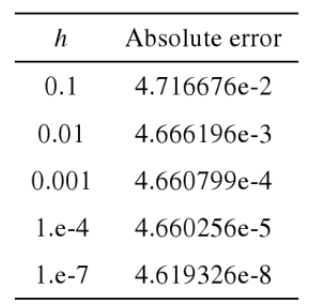
\includegraphics[width=6cm]{good.png}
  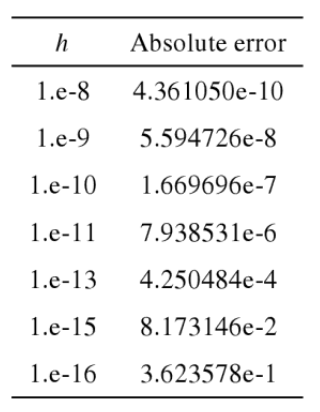
\includegraphics[width=5cm]{bad.png}
  
\end{note}

\begin{note}
  In practice, error is the sum of \vocab{discretization error} + \vocab{rounding error}
\end{note}

\subsection{Algorithm Properties}

Some good assessments of the quality of an algorithm are accuracy, efficiency, and robustness

\begin{definition}[Accumulated Error]
  Suppose you're evaluating polynomial with large degree. Your error $e_1$ from $p_1$ gets compounded 
  by $e_2$ from $p_2$ and so on and so forth, so the total error follows
  \[\text{Total error } \leq |e_1| + \cdots + |e_n|\]
\end{definition}

\section{Binary Representation, Rounding Errors, Truncation Errors}

\begin{remark}
  Math claim: Any real number $x \in \RR$ is accurately representable by an infinite sequence of digits, eg. $x \approx \pm 1$
  \[x = \pm c(1.\{d_1\}\ldots\{d_{t+1}\}\cdots) \times 2^e\]
  where $d_1, d_2, \cdots$ are integer numbers $0$ or $1$, and $e$ is the integer exponent.

  For each $e$, you can find a sequence to represent this real number $x$. 
\end{remark}

\begin{example}
  Let $x = -(1.10110\cdots) \times 2^1$ which means $x = -1 + 1 \times \frac{1}{2} + 0 \times \frac{1}{2^2} + 1 \times \frac{1}{2^3} + \cdots$
  where the $\frac{1}{2^t}$ term, we denote as $\frac{1}{s^t}$
\end{example}

\begin{definition}[Truncating]
  Chopping ignores digits $d_t, d_{t+1}, \cdots$ yielding $\overset{\sim}{x} = \pm (1.\{d_1\}\cdots\{d_{t-1}\}) \times 2^e \approx x$
  and so the error is $\O(\frac{1}{2^{te}}) = \O(\frac{1}{s^t})$
\end{definition}

\begin{definition}[Rounding]
  
\end{definition}

\end{document}

